\documentclass[a4paper, 14pt]{article}
\usepackage[utf8]{inputenc}
\usepackage[russian]{babel}
\usepackage{graphicx}
\usepackage{listings}
\usepackage{color}
\usepackage{amsmath}
\usepackage{pgfplots}
\usepackage{url}
% подключаем hyperref (для ссылок внутри  pdf)
\usepackage[unicode, pdftex]{hyperref}
\usepackage[T2A]{fontenc}
\usepackage[utf8]{inputenc}
\lstset{tabsize=2,
    breaklines,
    columns=fullflexible,
    flexiblecolumns,
    numbers=left,
    keepspaces=true,
    numberstyle={\footnotesize},
    extendedchars=\true
}
\lstdefinelanguage{MyC}{
  language=C++,
  ndkeywordstyle=\color{darkgray}\bfseries,
  identifierstyle=\color{black},
  morecomment=[n]{/**}{*/},
  commentstyle=\color{blue}\ttfamily,
  stringstyle=\color{red}\ttfamily,
  morestring=[b]",
  showstringspaces=false,
  morecomment=[l][\color{gray}]{//},
  keepspaces=true,
  escapechar=\%,
  %texcl=⟨true|false⟩
}
%\usepackage[russian,russian,english]{babel}
\frenchspacing                    % ставим пробелы в соответствии с французским стилем
\DeclareGraphicsExtensions{.pdf,.png,.jpg,.svg}
\usepackage{titlesec}
\usepackage[russian]{babel}
\usepackage{algpseudocode}
\usepackage{caption}
\usepackage{setspace}
\usepackage[linesnumbered,boxed]{algorithm2e}
\DeclareCaptionFont{white}{\color{white}} %% это сделает текст заголовка белым
%% код ниже нарисует серую рамочку вокруг заголовка кода.

\linespread{1}

\DeclareCaptionFormat{listing}{\colorbox{gray}{\parbox{\textwidth}{#1#2#3}}}
\captionsetup[lstlisting]{format=listing,labelfont=white,textfont=white} 

\begin{document}
	\begin{titlepage}
		\begin{center}
			\begin{LARGE}
				Отчет по лабораторной работе №5\\
					по курсу "Анализ алгоритмов"\\
					по теме "Распараллеливание вычислений"
			\end{LARGE}
		
			\begin{Large}
				\vspace{10cm}
				Студент: Доктор А.А. ИУ7-53\\
					Преподаватель: Волкова Л.Л.,
								   Строганов Ю.В.\\
				
				\vspace{5cm}2018 г.				   
			\end{Large}
			
		\end{center}
		 
	\end{titlepage}

\tableofcontents
	
\newpage
\section*{Введение}
\addcontentsline{toc}{section}{Введение}
\hspace{1cm}


Процесс с двумя потоками выполнения на одном процессоре
Пото́к выполне́ния (тред; от англ. thread — нить) — наименьшая единица обработки, исполнение которой может быть назначено ядром операционной системы. Реализация потоков выполнения и процессов в разных операционных системах отличается друг от друга, но в большинстве случаев поток выполнения находится внутри процесса. Несколько потоков выполнения могут существовать в рамках одного и того же процесса и совместно использовать ресурсы, такие как память, тогда как процессы не разделяют этих ресурсов. В частности, потоки выполнения разделяют инструкции процесса (его код) и его контекст (значения переменных, которые они имеют в любой момент времени). В качестве аналогии потоки выполнения процесса можно уподобить нескольким вместе работающим поварам. Все они готовят одно блюдо, читают одну и ту же кулинарную книгу с одним и тем же рецептом и следуют его указаниям, причём не обязательно все они читают на одной и той же странице \cite{multithreading_begin}.

На одном процессоре многопоточность обычно происходит путём временного мультиплексирования (как и в случае многозадачности): процессор переключается между разными потоками выполнения. Это переключение контекста обычно происходит достаточно часто, чтобы пользователь воспринимал выполнение потоков или задач как одновременное. В многопроцессорных и многоядерных системах потоки или задачи могут реально выполняться одновременно, при этом каждый процессор или ядро обрабатывает отдельный поток или задачу.

Потоки возникли в операционных системах как средство распараллеливания вычислений.

Параллельное выполнение нескольких работ в рамках одного интерактивного приложения повышает эффективность работы пользователя. Так, при работе с текстовым редактором желательно иметь возможность совмещать набор нового текста с такими продолжительными по времени операциями, как переформатирование значительной части текста, печать документа или его сохранение на локальном или удаленном диске. Еще одним примером необходимости распараллеливания является сетевой сервер баз данных. В этом случае параллелизм желателен как для обслуживания различных запросов к базе данных, так и для более быстрого выполнения отдельного запроса за счет одновременного просмотра различных записей базы. Именно для этих целей современные ОС предлагают механизм многопоточной обработки (multithreading). Понятию «поток» соответствует последовательный переход процессора от одной команды программы к другой. ОС распределяет процессорное время между потоками. Процессу ОС назначает адресное пространство и набор ресурсов, которые совместно используются всеми его потоками \cite{multithreading_history}.

Создание потоков требует от ОС меньших накладных расходов, чем процессов. В отличие от процессов, которые принадлежат разным, вообще говоря, конкурирующим приложениям, все потоки одного процесса всегда принадлежат одному приложению, поэтому ОС изолирует потоки в гораздо меньшей степени, нежели процессы в традиционной мультипрограммной системе. Все потоки одного процесса используют общие файлы, таймеры, устройства, одну и ту же область оперативной памяти, одно и то же адресное пространство. Это означает, что они разделяют одни и те же глобальные переменные. Поскольку каждый поток может иметь доступ к любому виртуальному адресу процесса, один поток может использовать стек другого потока. Между потоками одного процесса нет полной защиты, потому что, во-первых, это невозможно, а во-вторых, не нужно. Чтобы организовать взаимодействие и обмен данными, потокам вовсе не требуется обращаться к ОС, им достаточно использовать общую память — один поток записывает данные, а другой читает их. С другой стороны, потоки разных процессов по-прежнему хорошо защищены друг от друга.


\newpage
\section*{Задачи работы}

В ходе выполнения данной лабораторной работы, мной были выполнены следующие задачи:

\begin{enumerate}
\item[1)] научиться писать многопоточные программы;
\item[2)] применить полученные знания на практике, а именно переписать алгоритм Копперсмита — Винограда в несколько потоков;
\item[3)] провести замеры скорости работы однопоточной и многопоточной реализаций и проанализировать полученные результаты.
\end{enumerate}


\newpage
\section{Аналитическая часть}
\hspace{1cm}	В данном разделе приведено описание обычной реализации алгоритма Копперсмита — Винограда.

\subsection {Алгоритм умножения матриц Винограда} \\

Если посмотреть на результат умножения двух матриц, то видно, что каждый элемент в нем представляет собой скалярное произведение соответствующих строки и столбца исходных матриц. Можно заметить также, что такое умножение допускает предварительную обработку, позволяющую часть работы выполнить заранее. 
Рассмотрим два вектора

V = (v1, v2, v3, v4) и

W = (w1, w2, w3, w4).

Их скалярное произведение равно: 

V • W = v1w1 + v2w2 + v3w3 + v4w4.

Это равенство можно переписать в виде: 

V • W = (v1 + w2)(v2 + w1) + (v3 + w4)(v4 + w3) - v1v2 - v3v4 - w1w2 - w3w4.

 Кажется, что второе выражение задает больше работы, чем первое: вместо четырех умножений мы насчитываем их шесть, а вместо трех сложений - десять. Менее очевидно, что выражение в правой части последнего равенства допускает предварительную обработку: его части можно вычислить заранее и запомнить для каждой строки первой матрицы и для каждого столбца второй. На практике это означает, что над предварительно обработанными элементами нам придется выполнять лишь первые два умножения и последующие пять сложений, а также дополнительно два сложения.
\\

\normalsize \textbf {Улучшения алгоритма} \\

Возможны улучшения алгоритма с целью снизить его трудоемкость.

\begin{enumerate}
\item В 2010 Эндрю Стотерс усовершенствовал алгоритм до {\displaystyle O(n^{2.374}).}


\item В 2011 году Вирджиния Вильямс усовершенствовала алгоритм ещё раз — {\displaystyle O(n^{2.3728642}).}

\item В 2014 году Франсуа Ле Галль упростил метод Уильямса и получил новую улучшенную оценку {\displaystyle O(n^{2.3728639}).}

\end{enumerate}
	
		\newpage
	\section{Конструкторская часть}
	\hspace{1cm}В данном разделе размещены блоксхемы алгоритмов.
	\subsection{Разработка реализаций алгоритмов}
	
	\hspace{1cm}Ниже приложены блоксхемы алгоритмов решения поставленных задач
На рисунках \ref{ris:vin_good1} и \ref{ris:vin_good2} представлена реализация однопоточного алгоритма Винограда.

\begin{figure}[h]
\center
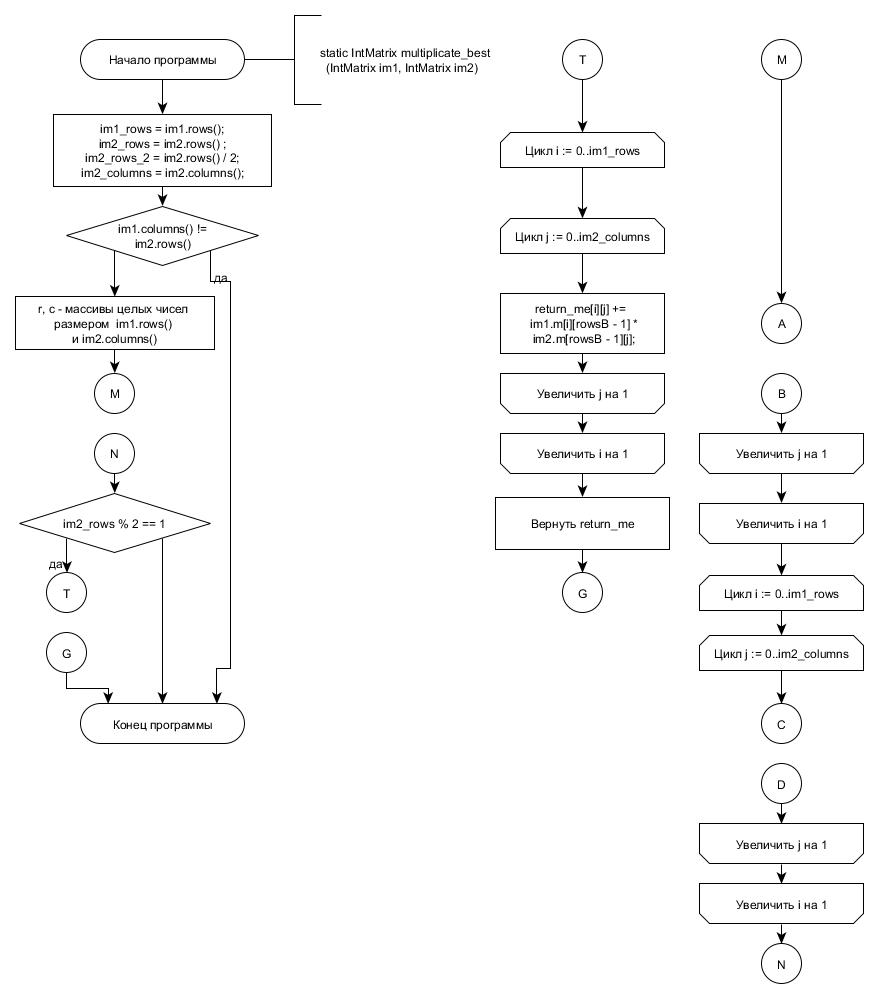
\includegraphics[scale=0.4]{vinograd_opt.jpg}
\caption{Виноград с оптимизациями, часть 1}
\label{ris:vin_good1}
\end{figure}

\begin{figure}[h]
\center
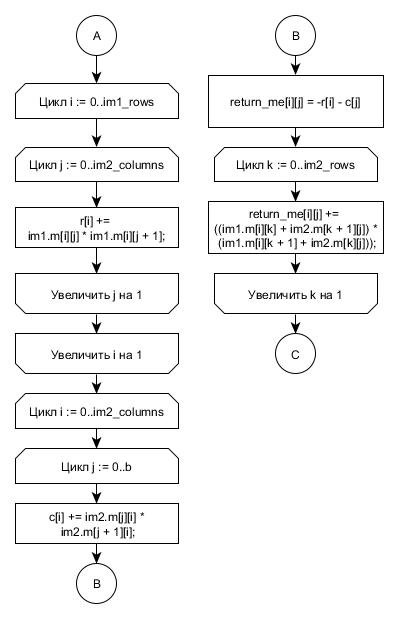
\includegraphics[scale=0.5]{vinograd_opt2.jpg}
\caption{Виноград с оптимизациями, часть 2}
\label{ris:vin_good2}
\end{figure}

	\newpage
	\section{Технологическая часть}
	\hspace{1cm}В данном разделе будут приведены:
	
    \begin{enumerate}
    \item[1)] средства реализации;
    \item[2)] листинг кода;
    \end{enumerate}

	\subsection{Средства реализации}
	\hspace{1cm}Для реализации программ мною был выбрал язык программирования - C++, поскольку имею опыт работы с ним. 
	Среда разработки - Qt.
	Для работы с потоками использовались библиотеки thread и mutex. Однако поскольку потоки не использовали разделяемую память, то использование семафоров не понадобилось, если не считать их использование в выводе данных для отладки. Для реализаций матриц использовалась библиотека vector
	Отключение оптимизации производилось с помощью директивы препроцессора
	#pragma optimize("", off). 
	Время работы процессора замерялось с помощью функции, продемонстрированной в листинге \ref{time}. Эта функция в отличие от встроенной функции таймера, способна считать реальное процессорное время работы программы в тиках \cite{lom}. Для ее работы была подключена библиотека time.h.
	\lstset{ %
        language=c++,                 % выбор языка для подсветки (здесь это С)
        basicstyle=\small\sffamily, % размер и начертание шрифта для подсветки кода
        numbers=left,               % где поставить нумерацию строк (слева\справа)
        numberstyle=\tiny,           % размер шрифта для номеров строк
        stepnumber=1,                   % размер шага между двумя номерами строк
        numbersep=-5pt,                % как далеко отстоят номера строк от         подсвечиваемого кода
        backgroundcolor=\color{white}, % цвет фона подсветки - используем         \usepackage{color}
        showspaces=false,            % показывать или нет пробелы специальными     отступами
        showstringspaces=false,      % показывать или нет пробелы в строках
        showtabs=false,             % показывать или нет табуляцию в строках
        frame=single,              % рисовать рамку вокруг кода
        tabsize=2,                 % размер табуляции по умолчанию равен 2 пробелам
        captionpos=t,              % позиция заголовка вверху [t] или внизу [b] 
        breaklines=true,           % автоматически переносить строки (да\нет)
        breakatwhitespace=false, % переносить строки только если есть пробел
        escapeinside={\%*}{*)},   % если нужно добавить комментарии в коде
	    keywordstyle=\color{blue}\ttfamily,
	    stringstyle=\color{red}\ttfamily,
	    commentstyle=\color{green}\ttfamily,
	    morecomment=[l][\color{magenta}]{\#},
	    columns=fullflexible
    }
	\begin{lstlisting}[label=time,caption=Функция замера процессороного времени]
    unsigned long long tick(void)
    {
        unsigned long long d;
        __asm__ __volatile__ ("rdtsc" : "=A"     (d));
        return d;
    }
	\end{lstlisting}

	\newpage
	\subsection{Реализация алгоритмов}
	
	В листинге \ref{vin} представлена реализация однопоточной реализации алгоритма.
	
	\begin{lstlisting}[label=vin,caption=Алгоритм Виноградова с оптимизациями]
  #pragma optimize("", off)
      static IntMatrix multiplicate_best(IntMatrix im1, IntMatrix im2) {

        if (im2.rows() != im1.columns())
            return (IntMatrix());
        IntMatrix return_me(im1.rows(), im2.columns());

        std::vector<int> r(im1.rows());
        std::vector<int> c(im2.columns());

        size_t im1_rows = im1.rows();
        size_t im2_rows_2 = im2.rows() / 2; 
        size_t im2_columns = im2.columns();

        for (size_t i = 0; i < im1_rows; i++) { 
            for (size_t j = 0; j < im2_rows_2; j++) { 
                r[i] += im1.m[i][j] * im1.m[i][j + 1]; 
            }
        }

        for (size_t i = 0; i < im2_columns; i++) {
            for (size_t j = 0; j < im2_rows_2; j++) { 
                c[i] += im2.m[j][i] * im2.m[j + 1][i];
            }
        }

        for (size_t i = 0; i < im1_rows; i++) { 
            return_me.m[i].clear(); 
            for (size_t j = 0; j < im2_columns; j++) { 
                return_me.m[i].push_back(0);
                return_me.m[i][j] = -r[i] - c[j];
                for (size_t k = 0; k < im2_rows_2; k++) {
                    return_me.m[i][j] += ((im1.m[i][k] + im2.m[k + 1][j]) *
                                          (im1.m[i][k + 1] + im2.m[k][j]));
                }
            }
        }

        size_t im2_rows = im2.rows();
        if (im2_rows % 2) { 
            for (size_t i = 0; i < im1_rows; i++) { 
                for (size_t j = 0; j < im2_columns; j++) {
                    im2_columns *
                    return_me.m[i][j] += im1.m[i][im2_rows - 1] * im2.m[im2_rows - 1][j];
                }
            }
        } 
        return return_me;
    }
	\end{lstlisting}
	
		Для реализации многопоточной реалиазация функция была разбита на 3 части. В листинге \ref{row} показана первая часть, отвечающая за создание вспомогательной строки. Вторая функция \ref{column} создает вспомогательный столбец. Непосредственно умножение матриц происходит в крайней функции \ref{umn}. 
	
	\begin{lstlisting}[label= row,caption=Создание вспомогательной строки]
      #pragma optimize("", off)
        void work_1_3(IntMatrix im1,
                      size_t im1_rows_begin,
                      size_t im1_rows, 
                      size_t im2_rows_2,
                      std::vector<int> &row){
             size_t i_begin = im1_rows_begin;
            size_t i_size = im1_rows;
            size_t j_size = im2_rows_2;
        
            for (size_t i = i_begin;u i < i_size; i++) {
                for (size_t j = 0; j < j_size; j++) {
                    row[i] += im1.m[i][j] * im1.m[i][j + 1];
                }
            }
        }
	\end{lstlisting}
	
		\begin{lstlisting}[label= column,caption=Создание вспомогательного столбца]
  #pragma optimize("", off)
    void work_2_3(IntMatrix im2,
                  size_t im2_columns_begin,
                  size_t im2_columns,
                  size_t im2_rows_2,
                  std::vector<int> &column){
        size_t i_begin = im2_columns_begin;
        size_t i_size = im2_columns;
        size_t j_size = im2_rows_2;
    
        for (size_t i = i_begin; i < i_size; i++) {
            for (size_t j = 0; j < j_size; j++) { 
                column[i] += im2.m[j][i] * im2.m[j + 1][i]; 
            }
        }
    }
	\end{lstlisting}
	
		\begin{lstlisting}[label= umn,caption= Перемножение матриц]
  #pragma optimize("", off)
void work_3_3(IntMatrix im1, IntMatrix im2,
              std::vector<int> c,
              std::vector<int> r,
              size_t im1_rows_begin,
              size_t im1_rows,
              size_t im2_columns,
              size_t im2_rows_2,
              IntMatrix &return_me)
{

    size_t im2_rows = im2.rows();
    size_t i_begin = im1_rows_begin;
    size_t i_size = im1_rows;
    size_t j_size = im2_columns;
    size_t k_size = im2_rows_2;

    for (size_t i = i_begin; i < i_size; i++) {
        return_me.m[i].clear();

        for (size_t j = 0; j < j_size; j++) {
            return_me.m[i].push_back(0);

            return_me.m[i][j] = -r[i] - c[j];

            for (size_t k = 0; k < k_size; k++) {
                return_me.m[i][j] += (
                            (im1.m[i][k] + im2.m[k + 1][j]) *
                            (im1.m[i][k + 1] + im2.m[k][j])
                        );
            }
            if (im2_rows % 2) {
                return_me.m[i][j] += im1.m[i][im2_rows - 1] *
                        im2.m[im2_rows - 1][j];
            }
        }
    }
}
	\end{lstlisting}
	
	\newpage
	В листинге \ref{multi2} представлена реализация двупоточной версии алгоритма. 4-ех, 6-и, 8-и поточные реализации сделаны аналогичным образом.
	
	\begin{lstlisting}[label=multi2,caption=Двупоточная реализация алгоритма Винограда]
       #pragma optimize("", off)
IntMatrix multi2(IntMatrix im1, IntMatrix im2) {

    if (im2.rows() != im1.columns())
        return (IntMatrix());

    IntMatrix return_me(im1.rows(), im2.columns());

    std::vector<int> r(im1.rows());
    std::vector<int> c(im2.columns());

    size_t im1_rows = im1.rows();
    size_t im2_rows_2 = im2.rows() / 2;
    size_t im2_columns = im2.columns();

    thread thread1_1(work_1_3,
                     im1, 
                     0, im1_rows,
                     im2_rows_2, 
                     ref(r));

    thread thread2_1(work_2_3, im2,
                     0, im2_columns,
                     im2_rows_2, 
                     ref(c));
    thread1_1.join();
    thread2_1.join();

    thread thread3_1(work_3_3, im1, im2
                     c, r, 0, im1_rows / 2, im2_columns, im2_rows_2,
                     ref(return_me));

    thread thread3_2(work_3_3, im1, im2,
                     c, r, im1_rows / 2, im1_rows, im2_columns, im2_rows_2,
                     ref(return_me)));

    thread3_1.join();
    thread3_2.join();

    return return_me;
}
	\end{lstlisting}
	
    \newpage
	\section{Экспериментальная часть}
	\hspace{1cm} В данном разделе будет сравнительный анализ реализаций алгоритма Винограда на основе экспериментальных данных. Во время проведения замеров использовался ноутбук c 2 физическими ядрами и 4 логическими процессорами.
    
      
    \subsection{Сравнительный анализ}
    \hspace{1cm}Для экспериментов использовались массивы, размер которых варьируется от 100 до 500 с шагом 100. 
    Количество повторов каждого эксперимента = 100. Результат одного эксперимента рассчитывается как средний из результатов проведенных испытаний с одинаковыми входными данными. Результаты замеров времени сведены в табл. \ref{tab:time}. Таблица состоит из 6 столбцов. Первый столбец представляет собой количество элементов. Второй - обычный оптимизированный алгоритм ВИнограда. Третий, четвертый, пятый и шестой - 2, 4, 6 и 8 поточные реализации. Те же результаты представлены на рис. \ref{grf:time}.

     
    \begin{table}[h]
        \caption{Результаты сравнения версий}
            \begin{tabular}{ | c | c | c | c | c | c | }
                \hline
                 Количество   &  1 поток   &  2 потока  &  4 потока &  6 потоков  &  8 потоков \\
                 элементов &  (в тиках) & (в тиках) & (в тиках) & (в тиках) & (в тиках) \\ \hline  
                  100 &    42120301  &    28547882  &    25954733  &    30014805  &    28076281 \\
                200 &    309628478  &    206121035  &    157828274  &    176815008  &    166488208 \\
                300 &    1018593267  &    640086297  &    518701316  &    556741606  &    571883017 \\
                400 &    2401139769  &    1483276424  &    1277150942  &    1295142955  &    1291652421 \\
                500 &    4670233016  &    2825425249  &    2442188430  &    2512812630  &    2486895374 \\
                \hline
            \end{tabular}
        \label{tab:time}
    \end{table} 
    
    
   \newpage  
    \begin{figure}
        \centering
        \includegraphics{}
       
    \begin{tikzpicture}
		\begin{axis}[
		    %title = ..  График времени работы реализаций алгоритма Винограда
		    xlabel={Размерность массива},
		    ylabel={Время в тиках},
		    ymin = 0, ymax = 4670233016,
		    legend pos=north west,
		    ymajorgrids=true,
		    grid style=dashed,
		]
		\legend{ 
	        один поток,
	        два потока,
	        четыре потока,
	        шесть потоков,
	        восемь потоков
	        }
  		\addplot[
  		    color=red,
  		    mark=square,
  		    ]
  		   coordinates {
  		    (100,42120301)
  		    (200,309628478)
  		    (300,1018593267)
  		    (400,2401139769)
			(500,4670233016)
  		    };

		\addplot[
  		    color=blue,
  		    mark=square,
  		    ]
  		    coordinates {
  		    (100,28547882)
  		    (200,206121035)
  		    (300,640086297)
  		    (400,1483276424)
			(500,2825425249)
  		    };
  		    
  	    \addplot[
  		    color=green,
  		    mark=square,
  		    ]
  		    coordinates {
  		    (100,25954733)
  		    (200,157828274)
  		    (300,518701316)
  		    (400,1277150942)
			(500,2442188430)
  		    };
  		 \addplot[
  		    color=purple,
  		    mark=square,
  		    ]
  		    coordinates {
  		    (100,30014805)
  		    (200,176815008)
  		    (300,556741606)
  		    (400,1295142955)
			(500,2512812630)
  		    };
  		\addplot[
  		    color=orange,
  		    mark=square,
  		    ]
  		    coordinates {
  		    (100,28076281)
  		    (200,166488208)
  		    (300,571883017)
  		    (400,1291652421)
			(500,2486895374)
  		    };
		\end{axis}
	\end{tikzpicture}
	 \caption{График версий алгоритма}
        \label{grf:time}
    \end{figure} 
	
    \newpage
	\section*{Вывод}
    \addcontentsline{toc}{section}{Вывод}
    
    
	\hspace{1cm} Как и ожидалось, многопоточные программы работают быстрее однопоточных решений, причем разница достигает почти двух раз(зависит от нагруженности процессора. Чем больше нагрузка, тем меньше эффективность нескольких потоков, поскольку им приходится простаивать в очереди). Наиболее эффективным количеством потоков оказалось число 4, равное количеству логических процессоров. При дальнейшим увеличении количества потоков увеличения скорости нет, зато увеличивается затрачиваемое время, что связано с издержками ожидания процессорного времени для потоков.
	\newpage
	\section*{Заключение}
    \addcontentsline{toc}{section}{Заключение}
    
	\hspace{1cm}В ходе работы были изучена и реализована многопоточность. Поскольку было выбрано разделение алгоритма так, чтобы не было разделяемой памяти, использования семафоров не было. Был сделан вывод, что наиболее оптимальное количество потоков в программе должно соотвествовать количеству логических процессоров используемого компьютера.
    
    \newpage

    \addcontentsline{toc}{section}{Список литературы}
    \begin{thebibliography}{11} 
    \bibitem{multithreading_begin}  kiranshobha01@gmail.com статья про устройство мультипоточности http://thekiransblog.blogspot.com/2010/02/multithreading.html
     \bibitem{multithreading_history}  Потоки и распараллеливание вычислений https://poznayka.org/s10704t1.html
    \bibitem{lom}И.В. Ломовской. Курс лекций по языку программирования C, 2017
    
    \end{thebibliography}

\end{document}